\documentclass[12pt,a4paper]{article}
\usepackage[margin=2cm]{geometry}
\usepackage{xeCJK}
\usepackage{fontspec}
\setCJKmainfont{Noto Serif CJK TC}[Script=CJK]
\usepackage{amsmath,amssymb}
\usepackage{graphicx}
\usepackage{fancyhdr}
\setlength{\headheight}{14.5pt}
\addtolength{\topmargin}{-2.5pt}
\usepackage{hyperref}
\usepackage{listings}
\usepackage{enumitem}
\usepackage{titlesec}
\usepackage{caption}
\usepackage{float}
\usepackage{indentfirst}
\setlength{\parindent}{2em}
\pagestyle{fancy}
\fancyhf{}
\cfoot{\thepage}
\linespread{1.3}

\title{暑期專題計劃書\\\large 肺部電腦斷層掃描之非小細胞癌 PD-L1 表現預測:\\結合多任務自監督學習與生成對抗網路}
\author{申請者:戴偉璿}
\begin{document}

\rhead{2025 年暑期專題}
\lhead{肺部電腦斷層掃描之非小細胞癌 PD-L1 表現預測}

\maketitle

\newpage

\section{研究背景}
PD-L1(Programmed Death Ligand 1)表現量是免疫治療中一個重要的生物標記,
常用以評估非小細胞肺癌(NSCLC)患者是否適合接受 PD-1/PD-L1 抑制劑。然而,
現有檢測方法依賴組織切片與免疫染色,具有侵入性、區域異質性與判讀主觀性等缺點。

以下是 PD-L1 表現的兩個例子,
50\% 是 NSCLC 中 PD-L1 表現的高低分界,>50\% 表示高表現,適合單藥免疫治療,預後較好;
<50\% 表示低表現,需聯合治療或非免疫療法,預後較差
\begin{figure}[h]
  \centering
  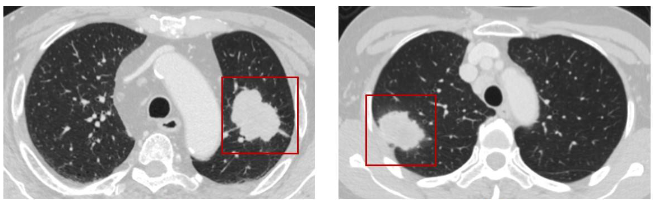
\includegraphics[width=0.8\textwidth]{src/image1.png}
  \centering
  \caption{左:PD-L1 表現>50\%;右:PD-L1 表現<50\%。圖片來源:周姵妤學姐碩士論文。}
  \label{fig:pdl1-examples}
\end{figure}

然而,隨著醫學影像技術的進步,肺部電腦斷層掃描(CT)已成為非小細胞肺癌診斷的重要工具。
但遇到了新的挑戰:樣本數量不足。相較於其他領域,醫學影像的取得尤為困難,
不只是因為需要專業的醫療設備與人員,還因為涉及患者隱私與倫理問題。
因此,如何在有限的資料條件下,準確預測 PD-L1 表現並且盡可能提昇模型的泛化能力,
成為一個亟待解決的問題。

近年來,自監督學習(Self-supervised Learning)的發展為解決資料稀缺問題提供了新的思路。
自監督學習通過從未標記的資料中學習有用的特徵表示,能夠在少量標記資料的情況下,
顯著提升模型性能。特別是多任務自監督學習(Multi-task Self-supervised Learning)方法,
通過同時學習多個相關任務,能夠進一步增強模型的表徵學習能力。

周姵妤學姐的碩士論文:「肺部電腦斷層掃描之非小細胞癌 PD-L1 表現預測 :
結合遮蓋圖像模型與生成對抗網路」中提出了一種基於 Masked autoencoder (MAE)
模型改良後的多模態模型 MTMAE , MAE 模型是一種自監督學習方法,
通過遮蔽部分輸入影像來學習有效的特徵表示。
學姐使用了實驗室之前研究出的 GAN 生成 CT 影像對模型進行預訓練,
並在微調階段使用真實的醫學影像進行訓練。該模型
結合了自監督重建、腫瘤分割與分類任務,
在低資料條件下有效提升了 PD-L1 表現的預測準確率。基於該模型的潛力,
我想嘗試看看這個方法能否有進一步改進的空間。

\begin{figure}[H]
  \centering
  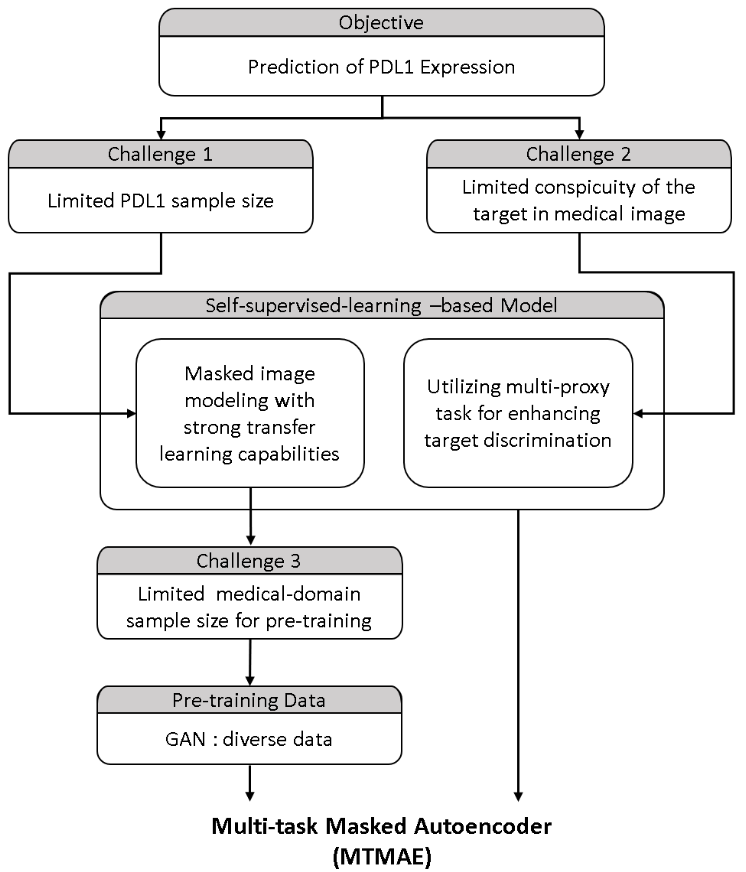
\includegraphics[width=0.8\textwidth]{src/image2.png}
  \centering
  \caption{MTMAE 模型架構。圖片來源:周姵妤學姐碩士論文。}
  \label{fig:MTMAE-model}
\end{figure}


\section{研究目標}
\begin{enumerate}
  \item 建立以 MTMAE 為基礎之 PD-L1 表現預測模型
  \item 探討加入對比學習對自監督表徵學習的增強效果。
  \item 在ViT encoder 中嵌入 GNN,建構 patch 間關聯性以提升特徵整合能力。
  \item 評估多模型集成(ensemble)策略對預測穩定性與泛化能力的影響。
\end{enumerate}

\newpage

\section{研究方法}
本研究將基於周姵妤學姐的碩士論文所提出的 MTMAE 模型進行改良,
模型核心為 Multi-task Masked Autoencoder(MTMAE) 。由於
影像資料的缺乏,我們先使用 GAΝ 生成批量的影像,對模型進行預訓練,接下來再使用
真正的醫學影像進行微調。

針對上述的研究目標,首先我將嘗試建立一個以 MTMAE 為基礎的 PD-L1 表現預測模型,
除了讓我熟悉 MTMAE 的架構外,這個基礎的模型也將作為後續改良的基準。

\subsection{對比學習}
對比學習是一種自監督學習方法,通過學習樣本之間的相似性與差異性來增強模型的表徵學習能力,
其擅長利用未標籤數據進行預訓練,減少對標籤數據的依賴。
本專題中,我將在 MTMAE 模型中加入對比學習模組,使用不同遮蔽策略產生的影像對作為正樣本,
以提升 encoder 對語意一致性的建模能力。這將有助於模型在少量標記資料的情況下,
學習到更豐富的特徵表示,從而提高 PD-L1 表現預測的準確性。

\subsection{GNN 結合}
圖神經網路(Graph Neural Network, GNN)是一種專門處理圖結構數據的深度學習模型,
能夠有效捕捉節點之間的關聯性與結構信息。
在本專題中,我將在 ViT encoder 中嵌入 GNN 模組,
將輸出的 patch token 建構為圖結構,節點間依位置或注意力建邊,
透過節點間的關聯性進行訊息傳遞,強化區域語意整合。
這將有助於提升模型對局部特徵的捕捉能力,進一步提高 PD-L1 表現預測的準確性。

\subsection{模型集成}
模型集成(Ensemble Learning)是一種通過結合多個模型的預測結果來提高整體性能的方法。
在本專題中,我將採用模型集成策略,利用隨機初始化、遮蔽方式或 GAN 輸入生成多個 MTMAE 模型,
最後透過投票的方式整合各模型的預測結果,以提升整體穩定性與泛化能力。
這種方法能夠減少單一模型的偏差與過擬合風險,從而提高 PD-L1 表現預測的穩定性。
除了原生的模型以外,我也會嘗試將對比學習、GNN 模組與集成模型結合,
以進一步提升預測效能。
\newpage

\section{實驗設計}

\subsection{實驗材料}

本專案預計使用來自於台大醫院、台大醫院新竹分院、台大醫院雲林分院提供之非小細胞肺癌患者 CT 與 PD-L1 標記資料做為輸入資料。
此外,為了解決資料稀缺問題,本專案也會使用實驗室先前所開發之 Gabor-GAN 模型,使用公開資料庫
LIDC-IDRT(Lung Image Database Consortium and Image Database Resource Initiative) 生成批量的樣本。

使用 GAN 生成的影像來訓練模型常面臨真實性的爭議,能夠生成準確的肺結節影像是關鍵。
為了控制生成影像的真實性(結核的大小以及形狀),我們使用結節分割標記引導生成。
流程包括:首先分割肺結節與肺實質背景,將背景與分割 mask 輸入 GAN,訓練生成肺結節樣本。
Gabor-loss GAN 使用 CNN 架構,訓練時除了真偽分類損失,還透過 Gabor filter 計算濾波特徵的損失(Gabor-loss),增強結節紋理並避免過擬合。
訓練完成後,使用肺部組織分割演算法提取肺實質背景,選取 64$\times$64$\times$64 的 VOI 作為輸入,將真實結節標記置於中間,
排除與肺壁、心臟等重疊的區域,並確保標記體積保留 80\% 以上。最後用高斯濾波器和平滑處理優化結節與背景的邊界。

藉由以上複雜的生成流程,我們期許能獲得高品質、高準確率的肺結節影像,增加模型預測的準確率。

\subsection{性能指標}

在判斷模型的預測效能時,我們將使用以下指標進行評估:
正確率(Accuracy)、靈敏度(Sensitivity)、  特異度(Specificity)與 AUC(Area under curve),
而這些指標的計算方式可由混淆矩陣得出(Confusion Matrix)得出,具體的混淆矩陣可分為四個象限:
\begin{itemize}
    \item 真陽性(True Positive, TP):模型正確預測為陽性的數量。
    \item 假陽性(False Positive, FP):模型錯誤預測為陽性的數量。
    \item 真陰性(True Negative, TN):模型正確預測為陰性的數量。
    \item 假陰性(False Negative, FN):模型錯誤預測為陰性的數量。
\end{itemize}

在本專題中,我們稍微修改了混淆矩陣的定義,
將陽性定義為 PD-L1 表現高於 50\% 的患者,陰性則為低於 50\% 的患者。

\begin{table}[h]
\centering
\begin{tabular}{|c|c|c|}
\hline
 & \textbf{實際陽性} & \textbf{實際陰性} \\ \hline
\textbf{預測陽性} & TP & FP \\ \hline
\textbf{預測陰性} & FN & TN \\ \hline
\end{tabular}
\caption{混淆矩陣}
\end{table}

藉由混淆矩陣,我們可以計算出以下指標:

\subsubsection{正確率(Accuracy)}
正確率是指模型正確預測的比例,在本專題中即正確分辨出 PD-L1 表現高於 50\% 與低於 50\% 的患者比例。
正確率是衡量模型整體預測準確性的指標,
計算公式為:
\begin{equation}
\text{Accuracy} = \frac{TP + TN}{TP + TN + FP + FN}
\end{equation}

\subsubsection{靈敏度(Sensitivity)}
靈敏度(也稱為召回率)是指模型正確預測為陽性的比例。在本專題中,靈敏度即預測 PD-L1 表現高於 50\% 的患者中,實際上也高於 50\% 的比例。
靈敏度是衡量模型對陽性樣本識別能力的指標,
計算公式為:
\begin{equation}
\text{Sensitivity} = \frac{TP}{TP + FN}
\end{equation}

\subsubsection{特異度(Specificity)}
特異度是指模型正確預測為陰性的比例。在本專題中,特異度即預測 PD-L1 表現低於 50\% 的患者中,實際上也低於 50\% 的比例。
特異度是衡量模型對陰性樣本識別能力的指標,
計算公式為:
\begin{equation}
\text{Specificity} = \frac{TN}{TN + FP}
\end{equation}
\subsubsection{AUC(Area under curve)}
AUC 是指 ROC 曲線下的面積,ROC 曲線是以假陽性率(False Positive Rate)為橫軸,真陽性率(True Positive Rate)為縱軸所繪製的曲線。
AUC 值介於 0 與 1 之間,值越大表示模型的預測能力越好。
計算公式為:
\begin{equation}
\text{AUC} = \int_{0}^{1} \text{TPR}(FPR) \, d(FPR)
\end{equation}

\begin{figure}[H]
  \centering
  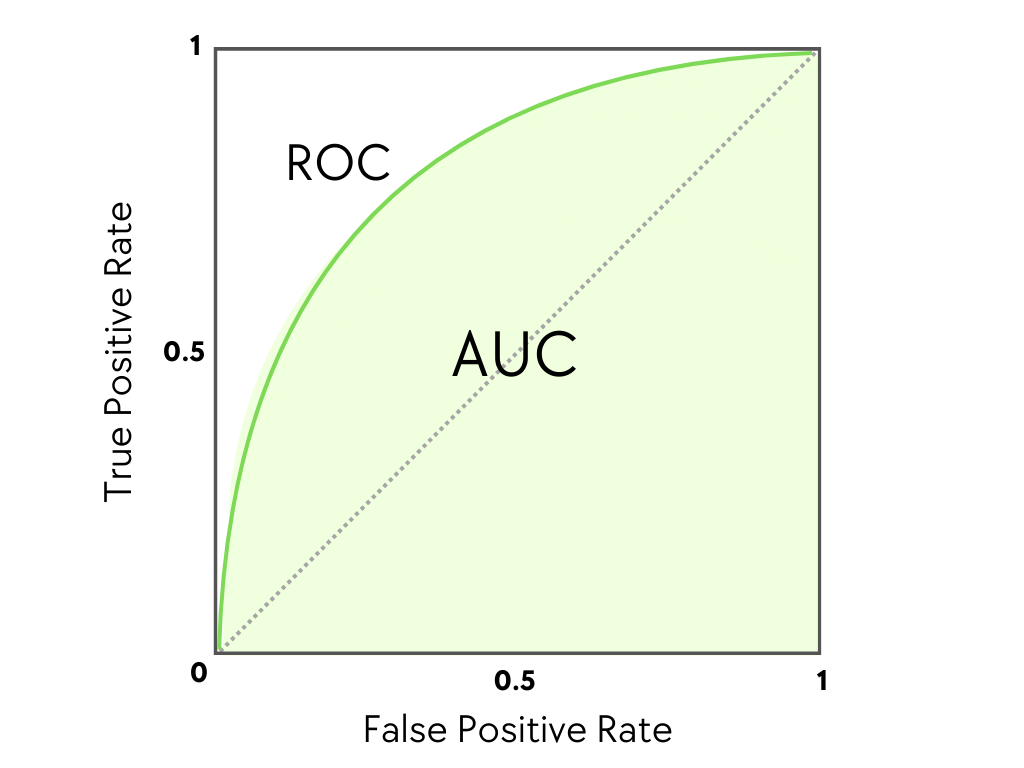
\includegraphics[width=0.8\textwidth]{src/image3.png}
  \centering
  \caption{ROC 曲線及其 AUC 值。}
  \label{fig:roc-curve}
\end{figure}
圖片來源:https://www.blog.trainindata.com/auc-roc-analysis/

\subsection{實驗方法}
本專題將使用 TensorFlow 框架實現 MTMAE 模型,並在此基礎上進行改良。
首先,我將建立一個基於 MTMAE 的 PD-L1 表現預測模型,並使用實驗室先前開發的 Gabor-GAN 生成 CT 影像進行預訓練。
接著,將使用真實的醫學影像進行微調,並在此基礎上嘗試加入對比學習模組、GNN 模組與模型集成策略。
在實驗過程中,我將使用 K-fold 交叉驗證方法來評估模型的泛化能力,
並使用上述的性能指標(正確率、靈敏度、特異度與 AUC)來評估模型的預測效能,同時比較不同改良方法對預測準確率的影響。

\section{預期成果}
根據論文內容,MTMAE 模型在 PD-L1 表現預測任務上的預測準確率僅為 0.724,然而,
若要達到臨床應用的標準,預測準確率需要達到 0.8 以上。
因此,本專題的目標是通過改良 MTMAE 模型,提升 PD-L1 表現預測的準確率。

針對上述提出的研究目標,本專題期許能將準確率進一步提升至 0.8 以上,
並且在靈敏度、特異度與 AUC 等指標上也能達到臨床應用的標準。
同時也驗證對比學習、GNN 以及模型集成等方法對於預測效能的提升效果。
期望透過這些改進能顯著提升模型的準確度與泛化能力。

\section{進度規劃}
\begin{tabular}{|c|c |l|  }
    \hline
    週次 & 日期 & 工作內容 \\
    \hline\hline
    1 & 6/16$\sim$6/22 & 閱讀論文、蒐集訓練資料、整理背景知識、建立 MTMAE 架構 \\
    \hline
    2$\sim$3 & 6/23$\sim$7/6 & 嘗試導入對比學習模組進行實驗 \\
    \hline
    4$\sim$5 & 7/7$\sim$7/20 & 嘗試加入 GNN 模組進行實驗 \\
    \hline
    6$\sim$7 & 7/21$\sim$8/3 & 嘗試集成模型進行實驗 \\
    \hline
    8 & 8/4$\sim$8/14 & 整理研究內容,撰寫書面報告 \\
    \hline
    9 & 8/15$\sim$8/21 & 完成最終簡報與口頭報告準備 \\
    \hline
\end{tabular}


\section{參考文獻}
\begin{enumerate}
    \item 周姵妤,肺部電腦斷層掃描之非小細胞癌 PD-L1 表現預測 :結合遮蓋圖像模型與生成對抗網路,碩士論文,國立臺灣大學,2024。
    \item PD-L1,https://en.wikipedia.org/wiki/PD-1\_and\_PD-L1\_inhibitors
    \item 自監督式學習,https://ithelp.ithome.com.tw/m/articles/10325328
    \item 對比學習,https://u9534056.medium.com/對比學習-Contrastive-Learning-主流方法一覽-bddf2afc5e5f
    \item 圖像神經網路,https://ithelp.ithome.com.tw/m/articles/10365828
    \item 交叉驗證,https://ithelp.ithome.com.tw/articles/10279240
    \item 混淆矩陣,https://ithelp.ithome.com.tw/articles/10254593
    \item 集成式學習,https://ithelp.ithome.com.tw/m/articles/10276102
\end{enumerate}
\end{document}